% ============================================================================
% Simulation study (transcribed from Zilan Chai's draft PDF, gBKMR_draft.pdf)
% ============================================================================

\section*{Simulation study}

We evaluate the ability of CausalBKMR to estimate the joint effect of a mixture in comparison to (i) the traditional regression approach with direct confounding adjustment in the outcome model, (ii) the parametric g-formula, (iii) the parametric g-formula with correct model specification, and (iv) BKMR with hierarchical variable selection grouped by time point (which ignores time-dependent confounding).

\subsection*{Setup}

A population dataset of $1{,}000{,}000$ observations was generated, where $\mathbf{A}_t = (A_{t,1}, \ldots, A_{t,k})^\top$ denotes the $k$-th metal exposure observed at the $t$-th time point. Baseline covariates $C_0$ and time-varying confounders $L_t$ were generated alongside. In each simulation, smaller datasets were randomly sampled from the population. Time-varying confounders were drawn from a normal distribution and log-transformed metal exposures from a multivariate normal distribution. Scenarios 1--4 considered two time points; scenarios 5--6 considered three time points (i.e., $t = 0, 1, 2$):
\begin{align*}
    \log A_0 &\sim N\!\left(h_{A_0}(C_0),\, \sigma^2_{A_0}\right), \\
    L_1 &\sim N\!\left(h_{L_1}(A_0, C_0),\, \sigma^2_{L_1}\right), \\
    \log A_1 &\sim N\!\left(h_{A_1}(A_0, L_1),\, \sigma^2_{A_1}\right), \\
    L_2 &\sim N\!\left(h_{L_2}(A_1, L_1),\, \sigma^2_{L_2}\right), \\
    \log A_2 &\sim N\!\left(h_{A_2}(A_1, L_2),\, \sigma^2_{A_2}\right).
\end{align*}

Two outcome types were considered, continuous and binary. The continuous outcome was generated by
\begin{equation*}
    y_i \sim N\!\left(h_Y(L_1, L_2, A_0, A_1, A_2),\, \sigma^2_Y\right),
\end{equation*}
and the binary outcome by
\begin{equation*}
    y_i \sim \text{Bin}\!\left(n,\, h_Y(L_1, L_2, A_0, A_1, A_2)\right).
\end{equation*}
Variances $\sigma^2_{A_t}$, $\sigma^2_{L_t}$, and $\sigma^2_Y$ were calibrated to be realistic based on the Strong Heart Study application. For the underlying exposure--confounder functions $h_{L_t}(\cdot)$ and exposure-response functions $h_{Y_t}(\cdot)$, we considered six scenarios for the continuous outcome and three additional scenarios for the binary outcome, varying linearity, strength of confounding, and presence of interactions. The specification of each scenario is summarised in Table~\ref{tab:sim_scenarios}.

\begin{table}[h]
\centering
\caption{Number of time points, the strength of the confounding effect, and exposure-confounder-response underlying relationships used for each simulation scenario.}
\label{tab:sim_scenarios}
\begin{tabular}{lccccc}
\toprule
Scenario & Time points & Correlation & Confounding & Underlying relationship & Outcome \\
\midrule
1 & 2 & moderate & low    & quadratic + interaction & continuous \\
2 & 2 & moderate & strong & linear                  & continuous \\
3 & 2 & moderate & strong & quadratic               & continuous \\
4 & 2 & moderate & low    & quadratic + interaction & binary     \\
5 & 3 & moderate & strong & quadratic               & binary     \\
6 & 3 & moderate & strong & linear                  & binary     \\
\bottomrule
\end{tabular}
\end{table}

For each scenario, $500$ datasets of $500$ observations were sampled from the population dataset. We first fit the BKMR confounder and outcome models:
\begin{align}
    L_{1i} &= h_L(\mathbf{A}_{0i}) + \mathbf{C}_i^\top \boldsymbol{\beta} + \epsilon_{L_{1i}}, \label{eq:sim_L1} \\
    L_{2i} &= h_L(\mathbf{A}_{0i}, \mathbf{A}_{1i}, \mathbf{L}_{1i}) + \mathbf{C}_i^\top \boldsymbol{\beta} + \epsilon_{L_{2i}}, \label{eq:sim_L2} \\
    Y_i &= h_Y(\mathbf{A}_{0i}, \mathbf{A}_{1i}, \mathbf{A}_{2i}, \mathbf{L}_{1i}, \mathbf{L}_{2i}) + \mathbf{C}_i^\top \boldsymbol{\theta} + \epsilon_{Y_i}. \label{eq:sim_Y}
\end{align}
Using CausalBKMR, we estimated the change in the potential outcome $Y$ for a shift of the exposure mixture from $\mathbf{a}$ (all exposures at the $25^{\text{th}}$ percentile of the underlying dataset) to $\mathbf{a}^*$ (all exposures at the $75^{\text{th}}$ percentile of the underlying dataset).

We compare the performance of the following six methods: (1) CausalBKMR with variable selection; (2) CausalBKMR without variable selection; (3) parametric g-formula with correct model specification; (4) traditional regression---linear or logistic regression with direct adjustment for all exposures and confounders at all time points; (5) parametric g-formula adjusting for all exposures and covariates; and (6) BKMR with hierarchical variable selection grouped by time points.

\subsection*{Simulation Results}

Tables~\ref{tab:sim_continuous} and~\ref{tab:sim_binary} summarise the empirical bias, mean squared error (MSE), and coverage probabilities of the average treatment effect estimates across the $500$ simulated datasets. Figure~\ref{fig:sim_results} visualises these results.

The parametric g-formula with correct model specification yielded low bias and high coverage, as expected. However, in real-world applications the true functional form is unknown, particularly when relationships involve quadratic terms or interactions; thus, although the correctly specified g-formula is a useful benchmark in simulation, its practical utility is limited. Traditional linear and logistic regression models exhibited substantial bias, particularly under nonlinear underlying relationships, because they cannot capture the time-varying structure of the data.

When the underlying relationship was linear (scenarios 2 and 6), coverage of the parametric g-formula was reasonable; otherwise (scenarios 1, 3, 4, 5), coverage dropped sharply, reflecting the heavy reliance of the parametric g-formula on correct model specification. CausalBKMR consistently exhibited low bias across scenarios, comparable to the correctly specified g-formula benchmark. CausalBKMR with and without variable selection produced similar bias and coverage in most cases; the no-selection variant slightly outperformed in some scenarios but at substantially higher computational cost (it estimates effects for all predictors rather than a selected subset). We therefore recommend CausalBKMR with variable selection in practice. BKMR with grouped variable selection exhibited the highest bias and lowest coverage among all methods, particularly under strong confounding, because it ignores time-varying confounding.

\begin{table}[h]
\centering
\caption{Bias, mean squared error (MSE), and coverage probabilities of the ATE estimates from our simulation under varying underlying relationships with a continuous outcome. Comparison of CausalBKMR with and without variable selection, the parametric g-formula, traditional linear regression, BKMR with grouped variable selection, and the parametric g-formula with correct model specification.}
\label{tab:sim_continuous}
\begin{tabular}{cl rrr}
\toprule
Scenario & Method & Bias & MSE & Coverage \\
\midrule
1 & CausalBKMR              &  0.00 & 0.01 & 0.98 \\
1 & g-formula               &  0.26 & 0.08 & 0.44 \\
1 & Linear model            &  0.26 & 0.08 & 0.47 \\
1 & BKMR-group              & $-0.02$ & 0.01 & 0.91 \\
1 & CausalBKMR (no varsel)  & $-0.00$ & 0.02 & 0.99 \\
1 & g-formula (correct)     &  0.01 & 0.01 & 0.93 \\
\midrule
2 & CausalBKMR              &  0.01 & 0.03 & 0.96 \\
2 & g-formula               & $-0.14$ & 0.04 & 0.84 \\
2 & Linear model            & $-0.14$ & 0.04 & 0.81 \\
2 & BKMR-group              & $-0.02$ & 0.63 & 0.01 \\
2 & CausalBKMR (no varsel)  & $-0.02$ & 0.04 & 0.99 \\
2 & g-formula (correct)     & $-0.00$ & 0.02 & 0.95 \\
\midrule
3 & CausalBKMR              & $-0.13$ & 0.05 & 0.91 \\
3 & g-formula               &  0.76 & 0.64 & 0.11 \\
3 & Linear model            & $-0.38$ & 0.25 & 0.78 \\
3 & BKMR-group              &  1.19 & 1.47 & 0.00 \\
3 & CausalBKMR (no varsel)  & $-0.11$ & 0.07 & 0.99 \\
3 & g-formula (correct)     &  0.09 & 0.03 & 0.95 \\
\bottomrule
\end{tabular}
\end{table}

\begin{table}[h]
\centering
\caption{Bias, mean squared error (MSE), and coverage probabilities of the ATE estimates from our simulation under varying underlying relationships with a binary outcome. Comparison of CausalBKMR with and without variable selection, the parametric g-formula, traditional logistic regression, BKMR with grouped selection, and the parametric g-formula with correct model specification.}
\label{tab:sim_binary}
\begin{tabular}{cl rrr}
\toprule
Scenario & Method & Bias & MSE & Coverage \\
\midrule
4 & CausalBKMR              &  0.03 & 0.00 & 0.77 \\
4 & g-formula               &  0.03 & 0.00 & 0.80 \\
4 & Linear model            & $-0.25$ & 0.09 & 0.68 \\
4 & BKMR-group              &  0.03 & 0.00 & 0.81 \\
4 & CausalBKMR (no varsel)  &  0.01 & 0.00 & 0.99 \\
4 & g-formula (correct)     & $-0.03$ & 0.00 & 0.83 \\
\midrule
5 & CausalBKMR              & $-0.02$ & 0.00 & 0.93 \\
5 & g-formula               &  0.08 & 0.14 & 0.78 \\
5 & Linear model            &  0.07 & 0.01 & 0.93 \\
5 & BKMR-group              &  0.08 & 0.01 & 0.45 \\
5 & CausalBKMR (no varsel)  &  0.01 & 0.00 & 0.97 \\
5 & g-formula (correct)     & $-0.02$ & 0.00 & 0.92 \\
\midrule
6 & CausalBKMR              & $-0.02$ & 0.00 & 0.94 \\
6 & g-formula               & $-0.10$ & 0.02 & 0.92 \\
6 & Linear model            &  0.04 & 0.01 & 0.95 \\
6 & BKMR-group              &  0.07 & 0.01 & 0.79 \\
6 & CausalBKMR (no varsel)  &  0.00 & 0.00 & 0.98 \\
6 & g-formula (correct)     & $-0.02$ & 0.00 & 0.93 \\
\bottomrule
\end{tabular}
\end{table}

\begin{figure}[h]
\centering
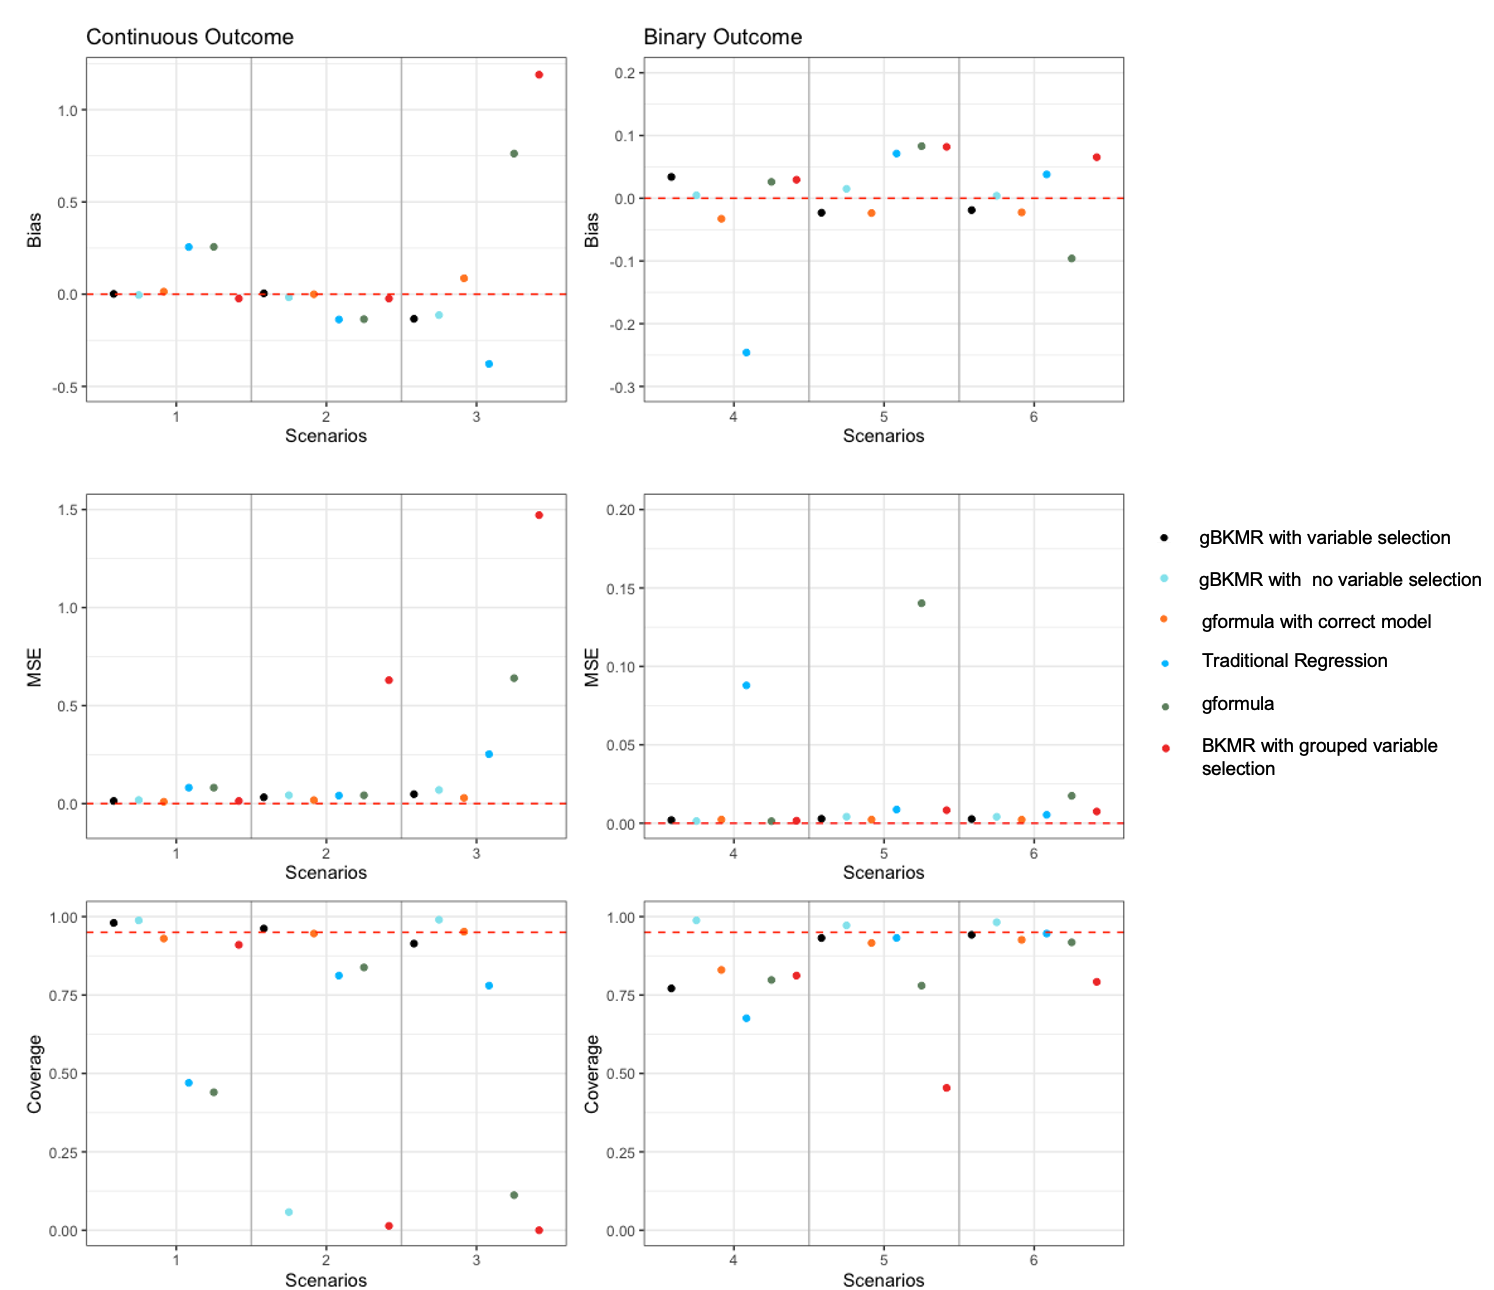
\includegraphics[width=0.95\textwidth]{figures/fig_simulation.png}
\caption{Bias, MSE, and coverage of the ATE estimates across the six simulation scenarios, comparing CausalBKMR (with and without variable selection) against the parametric g-formula, the parametric g-formula with correct model specification, traditional regression, and BKMR with grouped variable selection. Left column: continuous outcome (scenarios 1--3); right column: binary outcome (scenarios 4--6). Dashed red line indicates zero bias (top), zero MSE (middle), or nominal $95\%$ coverage (bottom).}
\label{fig:sim_results}
\end{figure}
